%!TEX root = ../thesis.tex

%%%%% Chapter: System Architecture %%%%%
\chapter{Alignment Algorithm}
\label{chap:align}

\ifpdf
    \graphicspath{{Chapter5/Figs/Raster/}{Chapter5/Figs/PDF/}{Chapter5/Figs/}}
\else
    \graphicspath{{Chapter5/Figs/Vector/}{Chapter5/Figs/}}
\fi


\section{Overview}

The use of the \texttt{diff}-based alignment algorithm in the system is inspired by the work \cite{lanchantin2015development} which used a \texttt{diff}-based algorithm to align imperfect captions to audio of TV shows. In fact, the \texttt{diff} algorithm (which solves the LCS problem) is a subset of a more general mathematical formulation of the 2-sequence alignment problem, which will be explained in \Cref{sec:diff-formulation} with enough detail. After the discussion of the general formulation, we will explain how to adapt this formulation to the real alignment algorithm used in the system. 

\section{General Formulation of Alignment Problems}
\label{sec:diff-formulation}

Let $X$ = $X_1^n$ = ($X_1$,$X_2$,\ldots,$X_n$) and $Y$ = $Y_1^n$ = ($Y_1$,$Y_2$,\ldots,$Y_m$) be two sequences of symbols where $X_i \in A$ and $Y_j \in B$ for all $i$ and $j$. The sets $A$ and $B$ are also called \textit{alphabets}. Let $\phi$ be the \textit{null symbol} which satisfies $\phi \notin A$ and $\phi \notin B$. Let $A^*$ = $A\cup\{\phi\}$ and $B^*$ = $B\cup\{\phi\}$.

Let $Z$ = $Z_1^p$ = ($Z_1$,$Z_2$,\ldots,$Z_p$), where $Z_i$ = $(S_i, T_i)$. Denote $S$ = $S_1^p$ = ($S_1$,$S_2$,\ldots,$S_p$) and $T$ = $T_1^p$ = ($T_1$,$T_2$,\ldots,$T_p$). We say $Z$ is an \textit{alignment} of sequences $X$ and $Y$ if:
\begin{enumerate}
  \item $Z_i \in A^* \times B^*$ and $Z_i \neq (\phi,\phi)$ for all $i$
  \item $X$ can be made equal to $S$ by inserting 0 or more null symbols $\phi$
  \item $Y$ can be made equal to $T$ by inserting 0 or more null symbols $\phi$
\end{enumerate}

Now define the \textit{Joint Weight Function}, $\mathcal{F}(\cdot,\cdot)$: $A^* \times B^* \to \mathbb{R}$. The \textit{optimal alignment} $Z_{opt}$ is the alignment that maximise the sum of the joint weights, $\mathcal{W}$:
\begin{equation}
  Z_{opt} \,=\, \argmax_{Z} \mathcal{W}(Z) \,=\, \argmax_{Z} \sum_{i=1}^{p} \mathcal{F}(S_i,T_i)
\end{equation}
where $p$ denotes the length of $Z$ and may vary when $Z$ changes. The optimal alignment could be found by the \textit{Needleman-Wunsch Algorithm}~\cite{needleman1970general} with time and space complexity $O(nm)$.

\section{Example: DNA Sequences}

In bioinformatics we often need to align different DNA sequences. To illustrate the above formulation, we use two example DNA sequences $X$ = \texttt{GCATGCT} and $Y$ = \texttt{GATTACA} with alphabets $A$ = $B$ = \{\texttt{A}, \texttt{T}, \texttt{G}, \texttt{C}\}. An example alignment could be:
\begin{center}
  \texttt{GCATG-CT}\\
  \texttt{G-ATTACA}
\end{center}
we can use $Z$ = (
  (\texttt{G},\texttt{G}),
  (\texttt{C},$\phi$),
  (\texttt{A},\texttt{A}),
  (\texttt{T},\texttt{T}),
  (\texttt{G},\texttt{T}),
  ($\phi$,\texttt{A}),
  (\texttt{C},\texttt{C}),
  (\texttt{T},\texttt{A})
) to express this alignment using the formulation in \Cref{sec:diff-formulation}.

Usually when comparing two sequences, we care about the total weight (or score) of converting the first sequence to the second sequence by three basic operations: \textit{insertion}, \textit{deletion} and \textit{substitution}. These could be actually reflected in the Joint Weight Function $\mathcal{F}$:
\[
  \begin{cases}
    \mathcal{F}(\phi,y) & \text{\quad insert } y \text{ into } X \\
    \mathcal{F}(x,\phi) & \text{\quad delete } x \text{ from } X \\
    \mathcal{F}(x,y) & \text{\quad substitute } x \text{ with } y
  \end{cases}
\]
In the alignment of DNA sequences, it is common to assign positive scores for matches (same symbols) and negative scores for mismatches (insertions, deletions, substitutions with different symbols). If we define $\mathcal{F}(x,y)$ to be +1 if $x$ = $y$ and -1 otherwise, the total weight (or score) $\mathcal{W}$ can be calculated as:
\[ \mathcal{W}(Z) = + 1 - 1 + 1 + 1 - 1 - 1 + 1 - 1 = 0 \]

\section{Alignment in the System}
\label{sec:align-in-system}

In our system, we need to find the alignment between chunks of the handout text and segments of the lecture audio file. As a first step, we define $X$ to be the sequence of extracted words in the handout and define $Y$ to be the sequence of transcribed words in the corresponding audio file.

We can now define our Joint Weight Function $\mathcal{F}$. For the baseline alignment algorithm, the optimal alignment of $X$ and $Y$ just solves the \textit{longest common subsequence} problem, like the original \texttt{diff} algorithm. This is equivalent to using the following simple JWF:
\begin{equation}
  \mathcal{F}(x,y) = 
  \begin{cases}
    1 & \text{if } x = y\\
    0 & \text{otherwise}
  \end{cases}
  \label{eq:jwf-baseline}
\end{equation}
The optimal alignment $Z_{opt}$ could then be found with the JWF in \Cref{eq:jwf-baseline}.

As a next step, we should notice that each word in $X$ links to a unique chunk ID in the handout and each word in $Y$ is associated with a starting timestamp in the audio file. These information can be combined with the optimal alignment of $X$ and $Y$ to assign a time interval to each chunk of the handout.

\begin{figure}[!tb]
  \centering
  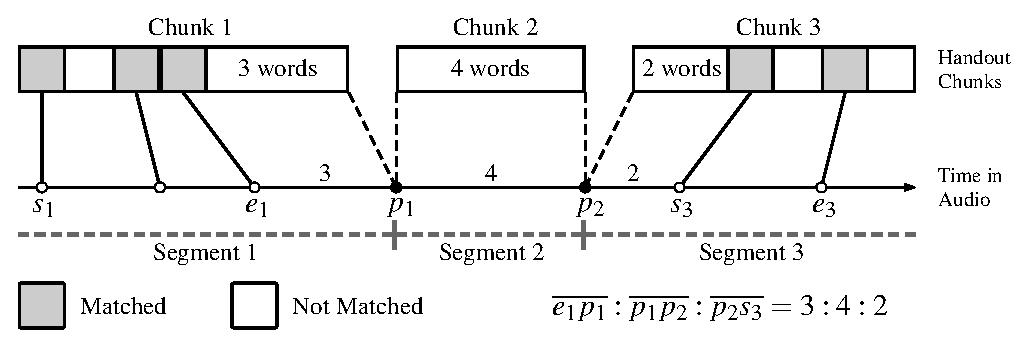
\includegraphics[width=.9\textwidth]{align-algo-fig.eps}
  \caption{Illustration of how to assign audio segments to handout chunks with the optimal alignment $Z_{opt}$}
  \label{fig:align-algo-fig}
\end{figure}

\Cref{fig:align-algo-fig} illustrates the strategy of assigning audio segments to handout chunks based on the optimal alignment $Z_{opt}$. The word matches in $Z_{opt}$ are indicated by solid lines between words in handout chunks and the points on the audio timeline. Chunk 1, 2, 3 have 3, 0, 2 matches respectively.

First we assign $\overline{s_1 e_1}$ and $\overline{s_3 e_3}$ to chunk 1 and chunk 3 respectively based on the matches. Then we divide $\overline{e_1 s_3}$ into three segments using two points $p_1$ and $p_2$ with ratio 3:4:2 based on these observations: there are 3 words between the last matched word and the last word in chunk 1; chunk 2 has no matches and has 4 words in total; there are 2 words between the first word and the first matched word in chunk 3. Finally, $p_1$ becomes the ending timestamp for chunk 1 and the starting timestamp for chunk 2, whilst $p_2$ becomes the ending timestamp for chunk 2 and the starting timestamp for chunk 3.

This strategy can be extended to any number of handout chunks. For each chunk with matches, the segment which corresponds to the first matched word and the last matched word is first assigned to this chunk. Then for each empty segment between the endpoints of the assigned segments, it is first divided into smaller segments based on the relative lengths (in number of words) of the unmatched words of the relevant handout chunks, and these smaller segments are then assigned to the corresponding chunks.

Note that this strategy is based on the assumption that the time spent on explaining a handout chunk is roughly proportional to the length of the chunk (in number of words).


\section{Extending the Baseline JWF}

Clearly the joint weight function can do more than just finding the longest common subsequence (\Cref{eq:jwf-baseline}) of two sequences. In this section we will discuss how the JWF could be extended in various ways.

\subsection{Adding Time Constraint}
\label{subsec:time-constraint}

Based on the assumptions that the lecturers will read the handouts in the strictly sequential order and that the amount of time spent on explaining a specific handout chunk is roughly proportional to the number of words in that chunk, we would expect that for any single match in the optimal alignment $Z_{opt}$, the difference between the relative position of the matching word in the handout and the relative position of the matching word in the audio file should be relatively small. 

Here we define the relative position of a word in the handout as the total number of its preceding words divided by the total number of words in the handout. Similarly we can define the the relative position of a word in the audio file to be the time difference between the timestamp of the word and the origin of the audio file, divided by the total length of the audio file. Clearly both of the relative positions range from 0 to 1.

In CUED the lectures are normally 50-minute long. Let $Z$ be a valid alignment and $(x,y)$ be an element in $Z$. Define $\mathcal{D}(x,y)$ as the difference between $x$'s relative position (in the handout) and $y$'s relative position (in the audio file) scaled by a factor of 50. We can interpret $\mathcal{D}(x,y)$ as the distance between $x$ and $y$ in minutes on the timeline of the audio file.

In the alignment algorithm, we would like to penalise large values of $\mathcal{D}(x,y)$. In the actual alignment system we use the Gaussian function with standard deviation $\sigma_t$, which yields the following JWF:
\begin{equation}
  \mathcal{F}(x,y) = 
  \begin{cases}
    \exp \left(-\frac{\mathcal{D}(x,y)}{2 \sigma_t^2}\right) & \text{if } x = y\\
    0 & \text{otherwise}
  \end{cases}
  \label{eq:jwf-gauss}
\end{equation}
we have removed the preceding normalising term of the Gaussian since it won't affect the optimal alignment. The Gaussian function decays when $\mathcal{D}(x,y)$ increases, which automatically penalises matches with large differences in relative positions.

\subsection{Penalising Common-word Matches}
\label{subsec:common-word-penalty}

In an alignment, matches of common words like `a', `the' and `it' should be assigned less weight than matches of other kinds of words. The Oxford Corpus have listed 100 most commonly used English words \cite{oec-common-words} based on the word frequencies in the corpus. Define the following function $\mathcal{C}(x)$ with a parameter $\alpha_c > 0$:
\begin{equation}
  \mathcal{C}(x) = 
  \begin{cases}
    \alpha_c & \text{if } x \text{ in the Oxford Corpus list}\\
    1 & \text{otherwise}
  \end{cases}
\end{equation}
Clearly $\alpha_c$ should be less than 1 in order to penalise common-word matches. Combining this function with \Cref{eq:jwf-gauss} yields the final JWF in the alignment algorithm:
\begin{equation}
  \mathcal{F}(x,y) = 
  \begin{cases}
    \mathcal{C}(x) \exp \left(-\frac{\mathcal{D}(x,y)}{2 \sigma_t^2}\right) & \text{if } x = y\\
    0 & \text{otherwise}
  \end{cases}
  \label{eq:jwf-final}
\end{equation}
note that the final $\mathcal{F}(x,y)$ has two adjustable parameters $\sigma_t$ and $\alpha_c$.


\nomenclature[z-JWF]{JWF}{Joint Weight Function}
\nomenclature[g-nullsymb]{$\phi$}{null symbol in sequence alignment}
\nomenclature[x-jwf]{$\mathcal{F}(x,y)$}{joint weight function with input symbols $x$ and $y$}
\nomenclature[x-sigma]{$\sigma_t$}{Gaussian standard deviation for adding time constraint}
\nomenclature[x-alpha]{$\alpha_c$}{coefficient for penalising common-word matches}